\documentclass[10pt,a4paper]{article}
\usepackage[margin=20mm]{geometry}
\usepackage{graphicx}
\usepackage{caption}
\usepackage[hidelinks]{hyperref}
\hypersetup{pdftitle={A.D.A.P.T. Supplementary Figures},pdfauthor={}}
\begin{document}
\begin{center}\Large A.D.A.P.T.: Supplementary Figures\end{center}
\noindent These figures accompany the existing journal manuscript. Each panel is generated from recorded experiment results; simulated operators and SITL are identified in the captions.
\begin{figure}[h!]\centering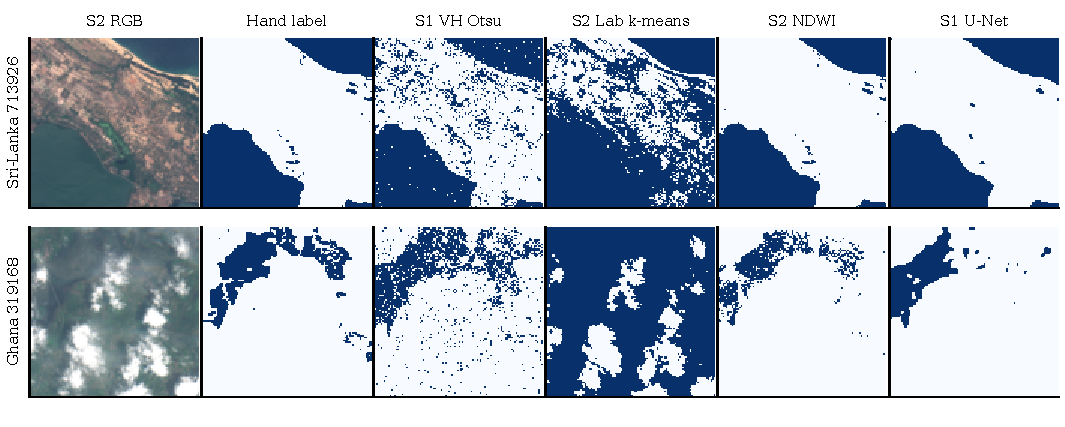
\includegraphics[width=.96\textwidth]{figures/fig_segmentation_qual.pdf}\caption*{\textbf{S1.} Held-out Sen1Floods11 examples. The hand label is an evaluation target; S1 and S2 methods use different inputs.}\end{figure}
\begin{figure}[h!]\centering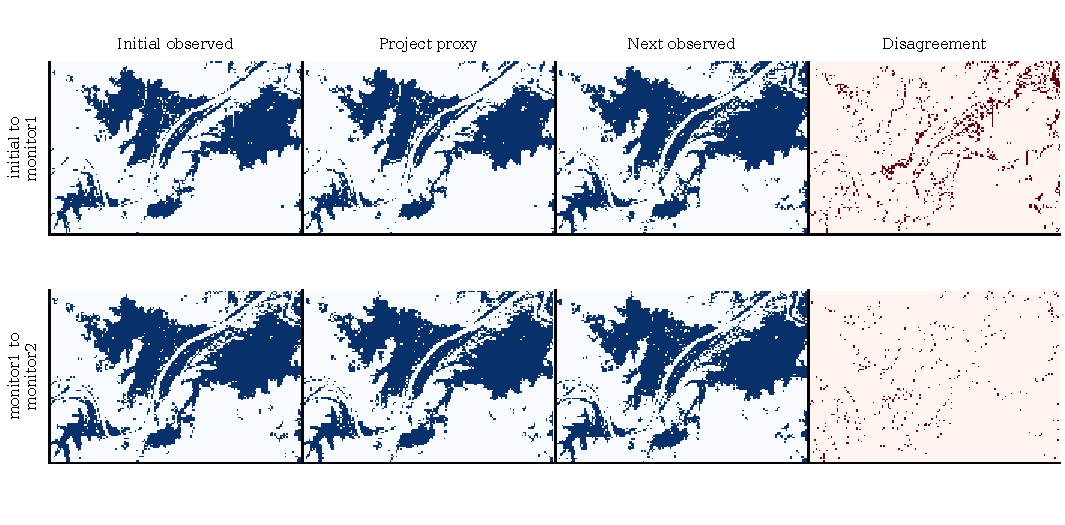
\includegraphics[width=.96\textwidth]{figures/fig_forecast_observed.pdf}\caption*{\textbf{S2.} Observed EMS flood progressions compared with the unchanged project proxy. Both comparisons tie persistence.}\end{figure}
\begin{figure}[h!]\centering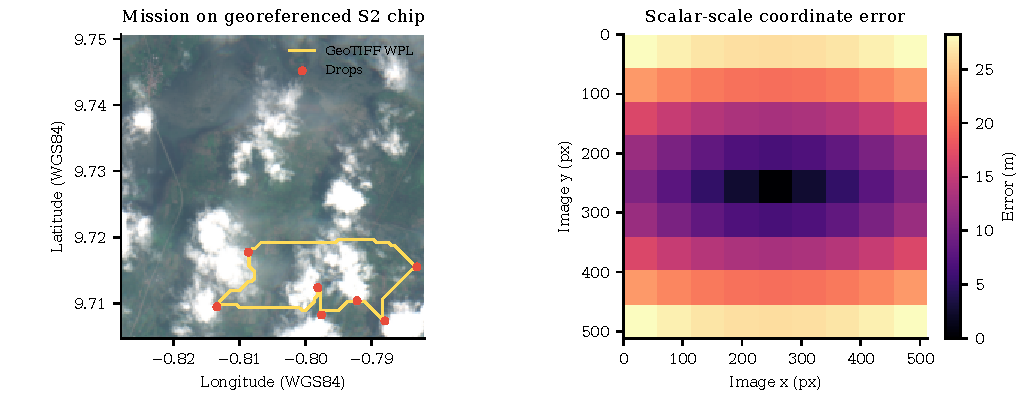
\includegraphics[width=.96\textwidth]{figures/fig_georeferenced_mission.pdf}\caption*{\textbf{S3.} Label-rendered diagnostic route on a co-registered satellite chip and scalar coordinate error. This is not flight validation.}\end{figure}
\clearpage
\begin{figure}[h!]\centering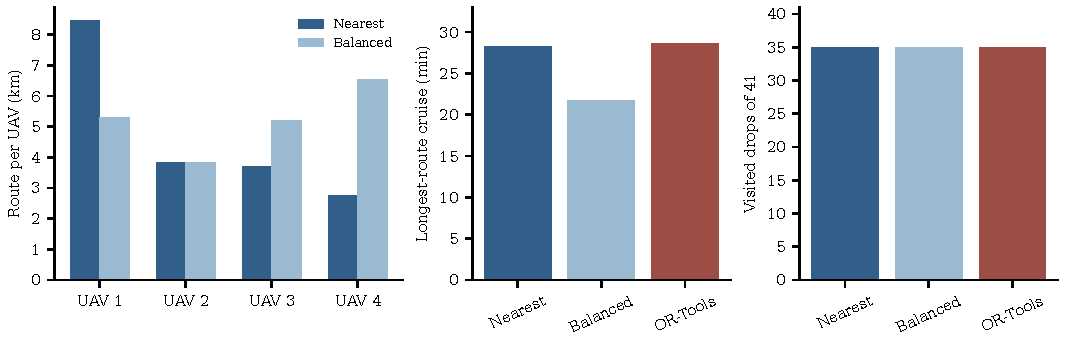
\includegraphics[width=.96\textwidth]{figures/fig_workload_vrp.pdf}\caption*{\textbf{S4.} Nearest-feasible, balanced and OR-Tools allocation comparisons. Times are optimistic route-length/speed proxies.}\end{figure}
\begin{figure}[h!]\centering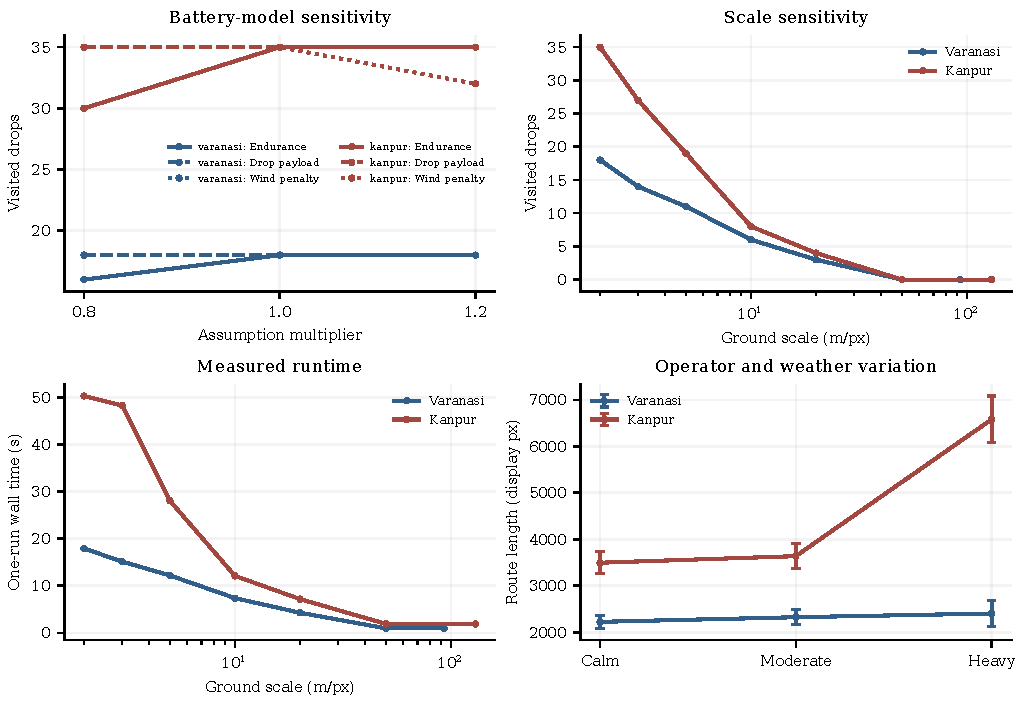
\includegraphics[width=.96\textwidth]{figures/fig_sensitivity_suite.pdf}\caption*{\textbf{S5.} Battery-model, scale, runtime and simulated-operator/weather sensitivity.}\end{figure}
\begin{figure}[h!]\centering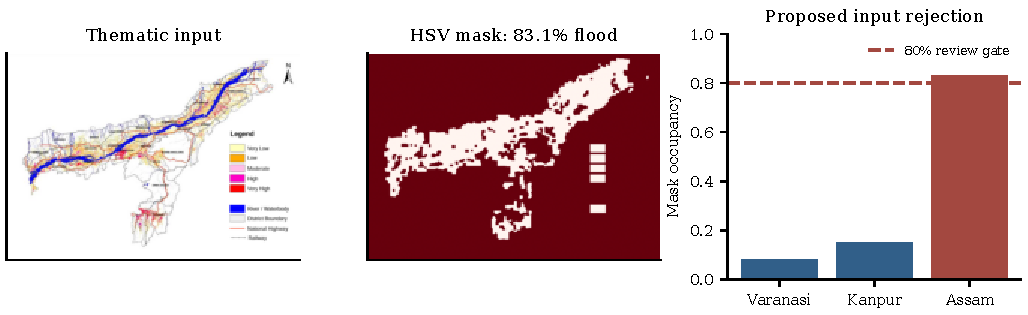
\includegraphics[width=.96\textwidth]{figures/fig_assam_failure.pdf}\caption*{\textbf{S6.} Assam thematic input, erroneous HSV flood mask and optional 80\% rejection guard.}\end{figure}
\begin{figure}[h!]\centering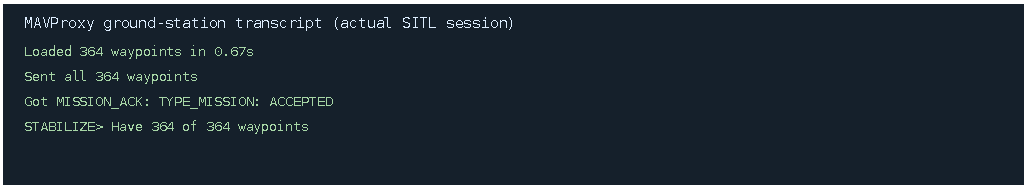
\includegraphics[width=.96\textwidth]{figures/fig_mavproxy.pdf}\caption*{\textbf{S7.} Actual MAVProxy command-line ground-station transcript during the full WPL upload to ArduCopter SITL.}\end{figure}
\end{document}
